%% ============================================================
%%  Second Review Report - FYP
%%  Physics-Informed Gait Modeling for Freezing-of-Gait Detection
%%  Department of Instrumentation and Control Engineering
%%  National Institute of Technology Tiruchirappalli
%% ============================================================
%%
%%  OVERLEAF INSTRUCTIONS
%%  1. Create a new Overleaf project and upload this as main.tex
%%  2. Set Compiler to pdfLaTeX (Menu -> Compiler -> pdfLaTeX)
%%  3. Logo: upload NITT_Logo.png and update the path below
%%  4. Figures: upload phase_portraits.png, radius_collapse.png,
%%     fogi_trajectory.png, cross_dataset_comparison.png from results/figures/
%% ============================================================

\documentclass[12pt,a4paper]{article}

%% ---- Packages ----
\usepackage[a4paper, top=3.8cm, bottom=2.5cm, left=2.5cm, right=2.5cm]{geometry}
\usepackage{graphicx}
\usepackage{amsmath,amssymb}
\usepackage{fancyhdr}
\usepackage{titlesec}
\usepackage{booktabs}
\usepackage{array}
\usepackage{multirow}
\usepackage{enumitem}
\usepackage{setspace}
\usepackage{parskip}
\usepackage{xcolor}
\usepackage{cite}
\usepackage{adjustbox}
\usepackage[hidelinks,colorlinks=true,linkcolor=black,urlcolor=blue,citecolor=black]{hyperref}

%% ---- TikZ & PGFPlots ----
\usepackage{tikz}
\usepackage{pgfplots}
\pgfplotsset{compat=1.18}
\usetikzlibrary{shapes.geometric,arrows.meta,positioning,fit,
                decorations.pathreplacing,calc,patterns,backgrounds}

%% ---- Colours ----
\definecolor{blockblue}{RGB}{52,101,164}
\definecolor{blockorange}{RGB}{206,92,0}
\definecolor{blockgreen}{RGB}{78,153,78}
\definecolor{blockgray}{RGB}{120,120,120}
\definecolor{lightblue}{RGB}{220,234,255}
\definecolor{lightorange}{RGB}{255,238,210}
\definecolor{lightgreen}{RGB}{220,245,220}
\definecolor{lightgray}{RGB}{240,240,240}
\definecolor{darkred}{RGB}{180,30,30}

%% ================================================================
%%  HEADER
%% ================================================================
\pagestyle{fancy}
\fancyhf{}
\fancyhead[C]{%
  \begin{tabular}{@{}l@{}}
    \begin{tabular}{@{}l@{\hspace{0.6em}}c@{}}
      \raisebox{-0.3\height}{%
        \includegraphics[height=1.8cm]{NITT Logo.png}
      }
      &
      \begin{tabular}[c]{@{}c@{}}
        \textbf{Department of Instrumentation and Control Engineering}\\[4pt]
        \textbf{National Institute of Technology Tiruchirappalli}
      \end{tabular}
    \end{tabular}\\[4pt]
    \rule{\textwidth}{0.4pt}
  \end{tabular}%
}
\fancyfoot[C]{\thepage}
\renewcommand{\headrulewidth}{0pt}
\setlength{\headheight}{52pt}
\addtolength{\topmargin}{-20pt}

%% ---- Section formatting ----
\titleformat{\section}{\large\bfseries}{}{0em}{}[\titlerule]
\titleformat{\subsection}{\normalsize\bfseries}{}{0em}{}
\titleformat{\subsubsection}{\normalsize\bfseries\itshape}{}{0em}{}

%% ================================================================
\begin{document}

%% ================================================================
%%  COVER PAGE
%% ================================================================
\thispagestyle{fancy}
\vspace*{1.5cm}

\begin{center}
  {\LARGE\textbf{\underline{Second Review Report}}}

  \vspace{1.2cm}
  \begin{minipage}{0.85\textwidth}
    \begin{flushleft}
      {\large\textbf{\underline{Title:}}}\\[6pt]
      \hspace{1em}\parbox{0.9\linewidth}{Physics-Informed Gait Modeling for Parkinson's Disease:
        Enhancing Early Warning of Freezing of Gait via Feature Fusion}
    \end{flushleft}
  \end{minipage}

  \vspace{1.0cm}
  \begin{minipage}{0.85\textwidth}
    \begin{flushleft}
      {\large\textbf{\underline{Guide's Name:}} Dr. D. Ezhilarasi}\\[6pt]
      \hspace{1em}%
    \end{flushleft}
  \end{minipage}

  \vspace{1.0cm}
  \begin{minipage}{0.85\textwidth}
    \begin{flushleft}
      {\large\textbf{\underline{Team Members:}}}
    \end{flushleft}
  \end{minipage}

  \vspace{0.5cm}
  \begin{tabular}{|p{3.8cm}|p{5cm}|p{5cm}|}
    \hline
    \textbf{Roll No} & \textbf{Name} & \textbf{Signature} \\
    \hline
    & & \\[2.2cm]
    \hline
  \end{tabular}
\end{center}

%% ================================================================
%%  PAGE 2 -- OBJECTIVES
%% ================================================================
\newpage
\section*{Objectives}

The objectives of this research have evolved from the fundamental modeling of gait dynamics
toward a robust, predictive framework for clinical application. The project aims to:

\begin{itemize}[leftmargin=*, itemsep=4pt]
  \item Develop a physics-informed modeling framework for human gait, enforcing smoothness,
        periodicity, and limit-cycle behaviour in the latent representation of wearable sensor
        data.
  \item Identify dynamical anomalies and phase-space stagnation as interpretable biomarkers for
        identifying Freezing of Gait (FoG), moving beyond generic black-box classification.
  \item Characterise the generalisability of rigid physics constraints and identify the
        limitations of latent ODE residuals in capturing patient-specific gait signatures.
  \item Refine the architecture toward \textbf{physics-informed feature fusion}, integrating
        empirically computed limit-cycle indicators and Early Warning Signals (EWS) to model
        the stochastic nature of freeze transitions.
  \item Shift the paradigm from event \emph{detection} to \textbf{early prediction}, targeting
        maximum predictive lead-times to identify impending freezes before they clinically
        manifest.
  \item Implement and evaluate a \textbf{three-stream CNN-LSTM fusion architecture} combining
        raw IMU signals, deterministic physics features, and EWS instability trends.
  \item Validate the resulting framework on independent cohorts (Daphnet, MJFF DeFOG) under
        strict 10-fold Leave-One-Subject-Out (LOSO) cross-validation to ensure clinical
        rigour and cross-dataset generalisability.
\end{itemize}

%% ================================================================
%%  WORK CARRIED OUT AFTER FIRST REVIEW
%% ================================================================
\newpage
\section*{Work Carried Out After First Review}

Following the first review, the project underwent a significant methodological pivot based on
experimental evidence. This section details the evolution from the initial approach to the final
architecture, the complete experimental results, and the analytical findings.

%% ---------------------------------------------------------------
\subsection*{1.\ Methodological Evolution: From PINN to Feature Fusion}

The first review presented a \textbf{GRU-PINN} architecture that modelled normal
gait as a limit cycle in a 2-D latent space and detected FoG as dynamical anomalies. During
extensive experimentation after the first review, we discovered that this rigid approach
\textbf{did not generalise well} across subjects. The key failure modes were:

\begin{enumerate}[leftmargin=*, itemsep=4pt]
  \item \textbf{Inter-subject variability:} No single set of ODE parameters could capture the
        diverse gait signatures across 10 patients.
  \item \textbf{Sensitivity loss:} Rigid dynamical constraints suppressed subtle, non-periodic
        precursors that often appear before FoG onset.
  \item \textbf{Optimisation instability:} Balancing data-loss and physics-residual weightings
        ($\lambda$) proved inconsistent across cross-validation folds.
\end{enumerate}

\vspace{4pt}

\noindent\textbf{Key scientific finding:} FoG is not a purely deterministic dynamical collapse;
it is a \textbf{stochastically driven transition} influenced by patient-specific physiological
noise. This led us to replace \emph{constraint-level} physics (rigid ODE residuals enforced in
the loss function) with \emph{feature-level} physics (empirically computed dynamical indicators
fed as auxiliary input streams).

\begin{figure}[ht]
\centering
\begin{adjustbox}{max width=\textwidth}

\begin{tikzpicture}[
  evobox/.style={draw, rounded corners=5pt, minimum width=3.8cm, minimum height=1.6cm,
                 align=center, font=\small, text width=3.6cm},
  arr/.style={-{Stealth[length=6pt]}, very thick},
  node distance=0.8cm
]
\node[evobox, fill=lightblue,   draw=blockblue, text=blockblue]   (r1)
  {\textbf{First Review}\\[2pt] Latent Neural ODE\\(PINN: rigid ODE\\constraints in loss)};
\node[evobox, fill=lightorange, draw=blockorange, text=blockorange, right=1.6cm of r1] (fail)
  {\textbf{Experimentation}\\[2pt] PINN fails on\\inter-subject\\variability};
\node[evobox, fill=lightgreen,  draw=blockgreen, text=blockgreen,  right=1.6cm of fail] (r2)
  {\textbf{Second Review}\\[2pt] 3-Stream Fusion\\(empirical physics\\features as inputs)};

\draw[arr, blockblue]   (r1.east)   -- (fail.west);
\draw[arr, blockorange] (fail.east) -- (r2.west);

\node[font=\scriptsize, text=darkred, below=0.15cm of fail]
  {\textit{AUC $\approx$ 0.77, insufficient}};
\node[font=\scriptsize, text=blockgreen, below=0.15cm of r2]
  {\textit{AUC = 0.871, Lead Time = 1.30\,s}};
\end{tikzpicture}
\end{adjustbox}
\caption{Methodological evolution from the first review (rigid PINN) to the second review
(feature-fusion architecture), driven by the experimental failure of constraint-level physics.}
\label{fig:evolution}
\end{figure}

%% ---------------------------------------------------------------
\subsection*{2.\ Revised System Architecture}

The final architecture is a \textbf{three-stream fusion network} that processes identical
preprocessed IMU windows through three parallel pathways before merging for prediction.

\begin{figure}[ht]
\centering
\begin{adjustbox}{max width=\textwidth}
\begin{tikzpicture}[
  sysbox/.style={draw, rounded corners=4pt, minimum height=0.8cm,
                 align=center, font=\small},
  bluebox/.style={sysbox, fill=lightblue,   draw=blockblue,   text=blockblue, minimum width=2.4cm},
  orangebox/.style={sysbox, fill=lightorange, draw=blockorange, text=blockorange, minimum width=2.4cm},
  greenbox/.style={sysbox, fill=lightgreen,  draw=blockgreen,  text=blockgreen, minimum width=2.4cm},
  graybox/.style={sysbox,  fill=lightgray,   draw=blockgray, minimum width=2.0cm},
  fusionbox/.style={sysbox, fill=yellow!20, draw=blockorange, text=black, minimum width=2.6cm,
                    minimum height=1.0cm, font=\small\bfseries},
  arr/.style={-{Stealth[length=5pt]}, thick},
  node distance=0.5cm and 0.7cm
]

%% Input
\node[graybox, minimum width=2.6cm] (inp) {IMU Window\\$128\times9$ @ 40\,Hz};

%% Stream 1: CNN-LSTM
\node[bluebox, above right=1.0cm and 2.0cm of inp] (cnn) {CNN Layers\\128$\to$64 filters};
\node[bluebox, right=0.5cm of cnn] (lstm) {LSTM\\64 hidden};

%% Stream 2: Physics
\node[orangebox, right=2.0cm of inp] (phys)
  {Physics Features\\FoGI, Radius, Phase\\Cadence, Energy};

%% Stream 3: EWS
\node[greenbox, below right=1.0cm and 2.0cm of inp] (ews)
  {EWS Features\\Var Trend, AR(1)\\Phase Vel., Entropy};

%% Arrows from input
\draw[arr] (inp.east) -- ++(0.6,0) |- (cnn.west);
\draw[arr] (inp.east) -- (phys.west);
\draw[arr] (inp.east) -- ++(0.6,0) |- (ews.west);

%% CNN to LSTM
\draw[arr] (cnn) -- (lstm);

%% Fusion block
\node[fusionbox, right=2.2cm of phys] (fuse) {Feature\\Concatenation\\(Dim = 96)};

\draw[arr] (lstm.east) -- ++(0.3,0) |- (fuse.west);
\draw[arr] (phys.east) -- (fuse.west);
\draw[arr] (ews.east) -- ++(0.3,0) |- (fuse.west);

%% FC layers
\node[graybox, right=0.6cm of fuse, minimum width=2.0cm] (fc) {FC Layers\\64$\to$32$\to$1};
\node[graybox, right=0.5cm of fc, minimum width=1.5cm, fill=lightgreen!50, draw=blockgreen]
  (out) {FoG\\Prediction};

\draw[arr] (fuse) -- (fc);
\draw[arr] (fc) -- (out);

%% Labels
\node[font=\scriptsize\bfseries, text=blockblue, above=0.05cm of cnn] {Stream 1: Raw IMU};
\node[font=\scriptsize\bfseries, text=blockorange, above=0.05cm of phys] {Stream 2: Physics};
\node[font=\scriptsize\bfseries, text=blockgreen, below=0.05cm of ews] {Stream 3: EWS};

\end{tikzpicture}
\end{adjustbox}
\caption{Three-stream fusion architecture. Stream~1 (blue) extracts temporal patterns via
CNN-LSTM. Stream~2 (orange) provides instantaneous physics features. Stream~3 (green) captures
instability trends. All streams are concatenated before fully connected classification layers.}
\label{fig:architecture}
\end{figure}

%% ---------------------------------------------------------------
\subsection*{3.\ Physics Feature Extraction}

The physics features are grounded in \textbf{nonlinear dynamical systems theory}, specifically the
modelling of gait as a periodic limit-cycle oscillator. We extract two categories of features:

\subsubsection*{3.1\ Limit-Cycle Indicators (Physics Stream)}

Using Takens' delay embedding theorem, we reconstruct a 2-D phase-space trajectory from the
ankle accelerometer signal:
\begin{equation}
  x_t = s(t),\quad y_t = s(t+\tau), \qquad \tau = 5 \text{ samples (0.125\,s)}
\end{equation}
From this embedding, we compute:

\begin{table}[ht]
\centering
\renewcommand{\arraystretch}{1.2}
\begin{adjustbox}{max width=\textwidth}
\begin{tabular}{p{3.2cm} p{5.5cm} p{5.5cm}}
\toprule
\textbf{Feature} & \textbf{Description} & \textbf{Metric Detail} \\
\midrule
Freezing Index (FoGI) & Power ratio 3--8\,Hz / 0.5--3\,Hz & Traditional spectral indicator \\
Dominant Frequency & Peak of the power spectral density (PSD) & Shift during trembling \\
Freeze Ratio & Power in freeze band / total power & Normalised spectral energy \\
Radius ($r_m$) & $L_2$ norm in $m$-dimensional state-space & Reconstructed attractor size \\
Radius mean/var & Windowed statistics of $r_t$ & Amplitude \& stability \\
Phase mean & Mean angular advance $\Delta\phi$ & Phase progression rate \\
Phase variance & Circular variance of phase $\theta_t$ & Periodicity regularity \\
Cadence regularity & Strongest autocorrelation peak (0.3--2\,s) & Stride timing consistency \\
Signal energy & RMS of filtered acceleration & Movement intensity \\
\bottomrule
\end{tabular}
\end{adjustbox}
\caption{Complete set of 9 physics features extracted from delay-embedded phase-space reconstruction.}
\label{tab:physics_features}
\end{table}

\subsubsection*{3.2\ Early Warning Signals (EWS Stream)}

Based on \textbf{critical transition theory} (Scheffer et al., 2009), these features detect
``critical slowing down,'' i.e.\ the gradual loss of attractor stability before a sudden collapse:

\begin{table}[ht]
\centering
\renewcommand{\arraystretch}{1.3}
\begin{adjustbox}{max width=\textwidth}
\begin{tabular}{p{3.5cm} p{5.0cm} p{5.5cm}}
\toprule
\textbf{EWS Feature} & \textbf{Computation} & \textbf{Rising Value Indicates} \\
\midrule
Radius variance trend & Variance of $r_t$ in 32-sample sub-windows &
  Growing fluctuations in limit-cycle diameter \\
AR(1) coefficient & Lag-1 autocorrelation of radius &
  Slower recovery from perturbations \\
Phase velocity drift & Std.\ dev.\ of $d\theta/dt$ &
  Inconsistent angular velocity around the attractor \\
FoGI slope & Linear trend of FoGI over window &
  Gradual buildup of freeze-band power \\
Spectral entropy & Entropy of power spectral distribution &
  Shift from periodic to broadband (chaotic) signal \\
\bottomrule
\end{tabular}
\end{adjustbox}
\caption{Early Warning Signal features derived from critical transition theory.}
\label{tab:ews_features}
\end{table}

%% ---------------------------------------------------------------
\newpage
\subsection*{4.\ Experimental Setup}

\subsubsection*{4.1\ Prediction Protocol}

Unlike the first review which focused on FoG \emph{detection} (classifying events as they occur),
we now target FoG \emph{prediction}: identifying an impending freeze \textbf{before onset}. This
is achieved by \textbf{shifting positive labels backward} by a prediction horizon $h$:
\begin{equation}
  \tilde{y}(t) =
  \begin{cases}
    1 & \text{if } \exists\; t' \in [t,\, t+h]: y(t')=\text{FoG} \\
    0 & \text{otherwise}
  \end{cases}
\end{equation}

We use $h = 1.6$\,s (2 windows at 0.8\,s stride) as the primary horizon. This means the model
must learn to detect \textbf{precursor signals} in the gait dynamics that occur up to 1.6 seconds
before the clinical freeze annotation.

\subsubsection*{4.2\ Cross-Validation Protocol}

Strict 10-fold Leave-One-Subject-Out (LOSO): in each fold, 8 subjects train, 1 validates
(threshold/early-stopping), 1 is tested. No test-subject data influence any statistics or
model selection. Subjects 4 and 10 have no FoG episodes and are excluded from AUC and lead-time
metrics ($n=8$ valid folds).

\subsubsection*{4.3\ Key Metrics}

\begin{itemize}[leftmargin=*, itemsep=3pt]
  \item \textbf{Lead Time:} time from the \emph{first} true-positive prediction to annotated FoG
        onset (median per fold; reported as Mean $\pm$ SD).
  \item \textbf{ROC-AUC:} threshold-independent discriminative performance.
  \item \textbf{Sensitivity / Specificity / F1-Score:} operating-point metrics at Youden's
        optimal threshold.
\end{itemize}

\subsubsection*{4.4\ Training and Preprocessing Configuration}

To ensure reproducibility, we detail the core technical configuration:
\begin{itemize}[leftmargin=*, itemsep=2pt]
  \item \textbf{Preprocessing:} Signals downsampled from 64\,Hz to 40\,Hz following an
        8th-order anti-aliasing Butterworth filter (cutoff = 20\,Hz).
  \item \textbf{Optimisation:} AdamW optimizer with $LR=10^{-3}$ and weight decay $10^{-5}$.
  \item \textbf{Scheduling:} Cosine annealing with $T_{max}=100$, batch size 1024, and
        gradient clipping (norm = 1.0).
  \item \textbf{Class Balancing:} Random oversampling of FoG windows (factor = 3) combined
        with weighted batch sampling.
  \item \textbf{Early Stopping:} Validation AUC monitored across folds with a patience of 15
        epochs.
\end{itemize}

%% ---------------------------------------------------------------
\subsection*{5.\ Complete Experimental Results}

\subsubsection*{5.1\ Daphnet Ablation Study (10-Fold LOSO)}

Table~\ref{tab:ablation} presents the core ablation comparing all model configurations. The
Freezing Index baseline and SVM baseline (using physics + EWS features) contextualise the
deep learning results.

\begin{table}[ht]
\centering
\caption{Daphnet ablation results (Mean $\pm$ SD across $n=8$ valid LOSO folds, $h=1.6$\,s).}
\label{tab:ablation}
\renewcommand{\arraystretch}{1.25}
\begin{adjustbox}{max width=\textwidth}
\begin{tabular}{llccccc}
\toprule
\textbf{Model} & \textbf{Streams} & \textbf{AUC} & \textbf{Lead (s)} & \textbf{Se} & \textbf{Sp} & \textbf{F1} \\
\midrule
Freezing Index & Classical & $0.746\!\pm\!0.067$ & $0.85\!\pm\!0.71$ & $0.581$ & $0.633$ & $0.295$ \\
SVM            & Physics+EWS & $0.823\!\pm\!0.098$ & $1.20\!\pm\!0.57$ & $0.590$ & $0.774$ & $0.359$ \\
\midrule
CNN--LSTM      & Raw IMU only  & $0.859\!\pm\!0.080$ & $1.05\!\pm\!0.53$ & $0.637$ & $0.856$ & $0.433$ \\
\textbf{Base + Physics} & Raw + Physics & $\mathbf{0.871\!\pm\!0.079}$ & $\mathbf{1.30\!\pm\!0.56}$ & $\mathbf{0.654}$ & $0.859$ & $0.451$ \\
Base + EWS     & Raw + EWS     & $0.858\!\pm\!0.054$ & $1.15\!\pm\!0.55$ & $0.632$ & $0.869$ & $0.446$ \\
Full Model     & All 3 streams & $0.869\!\pm\!0.059$ & $1.00\!\pm\!0.57$ & $0.619$ & $\mathbf{0.896}$ & $\mathbf{0.459}$ \\
\bottomrule
\end{tabular}
\end{adjustbox}
\end{table}

\vspace{6pt}

\noindent\textbf{Key observations:}
\begin{itemize}[leftmargin=*, itemsep=3pt]
  \item \textbf{Physics features extend early warning:} Base + Physics achieves the
        \textbf{longest lead time} (1.30\,s), a \textbf{+24\% improvement} over the pure
        CNN--LSTM baseline (1.05\,s).
  \item \textbf{Feature interference:} Adding EWS on top of physics (Full Model) \emph{reduces}
        lead time to 1.00\,s while improving specificity (0.896 vs 0.859). More features do not
        always mean earlier detection; they can shift the decision boundary toward precision.
  \item \textbf{Physics outperform SVM:} The deep fusion (AUC 0.871) surpasses the classical
        SVM baseline trained on the same features (AUC 0.823), confirming that \emph{learnable}
        integration of physics is superior to hand-crafted thresholds.
\end{itemize}

%% ---------------------------------------------------------------
\subsubsection*{5.2\ Visualising the Ablation}

Figure~\ref{fig:ablation_bar} displays the ablation results as a clustered bar chart for
intuitive comparison across all metrics.

%% ------- TikZ bar chart -------
\begin{figure}[ht]
\centering
\begin{adjustbox}{max width=\textwidth}
\begin{tikzpicture}
\begin{axis}[
  ybar=3pt,
  bar width=7pt,
  width=14cm, height=6cm,
  enlarge x limits=0.15,
  ylabel={Score},
  ylabel style={font=\small},
  symbolic x coords={FI Baseline, SVM, CNN-LSTM, Base+Phys, Base+EWS, Full Model},
  xtick=data,
  x tick label style={font=\small, rotate=20, anchor=east},
  ymin=0, ymax=1.05,
  legend style={font=\scriptsize, at={(0.5,1.05)}, anchor=south, legend columns=4},
  nodes near coords={\scriptsize\pgfmathprintnumber[fixed,precision=2]{\pgfplotspointmeta}},
  every node near coord/.append style={font=\tiny, rotate=90, anchor=west},
  grid=major,
  grid style={dashed, gray!30}
]
\addplot[fill=blockblue!70] coordinates
  {(FI Baseline,0.746) (SVM,0.823) (CNN-LSTM,0.859)
   (Base+Phys,0.871) (Base+EWS,0.858) (Full Model,0.869)};
\addplot[fill=blockorange!70] coordinates
  {(FI Baseline,0.581) (SVM,0.590) (CNN-LSTM,0.637)
   (Base+Phys,0.654) (Base+EWS,0.632) (Full Model,0.619)};
\addplot[fill=blockgreen!70] coordinates
  {(FI Baseline,0.633) (SVM,0.774) (CNN-LSTM,0.856)
   (Base+Phys,0.859) (Base+EWS,0.869) (Full Model,0.896)};
\addplot[fill=darkred!60] coordinates
  {(FI Baseline,0.295) (SVM,0.359) (CNN-LSTM,0.433)
   (Base+Phys,0.451) (Base+EWS,0.446) (Full Model,0.459)};
\legend{AUC, Sensitivity, Specificity, F1}
\end{axis}
\end{tikzpicture}
\end{adjustbox}
\caption{Clustered bar chart of ablation results across all model configurations on the Daphnet
dataset ($h=1.6$\,s, LOSO). Base+Physics achieves the best AUC and sensitivity; Full Model
achieves the highest specificity and F1 but at the cost of lead time.}
\label{fig:ablation_bar}
\end{figure}

%% ---------------------------------------------------------------
\newpage
\subsubsection*{5.3\ Per-Subject Performance (Base + Physics)}

The per-subject breakdown in Table~\ref{tab:persubj} reveals important heterogeneity in FoG
phenotypes.

\begin{table}[ht]
\centering
\caption{Per-subject results for the Base + Physics model (Daphnet, $h=1.6$\,s).}
\label{tab:persubj}
\renewcommand{\arraystretch}{1.25}
\begin{tabular}{cccc}
\toprule
\textbf{Subject} & \textbf{AUC} & \textbf{Sensitivity} & \textbf{Lead Time (s)} \\
\midrule
S01 & 0.929 & 0.873 & 1.60 \\
S02 & 0.949 & 0.938 & 1.60 \\
S03 & 0.887 & 0.855 & 1.60 \\
S04 & N/A {\scriptsize(no FoG)} & 0.000 & N/A \\
S05 & 0.914 & 0.835 & 1.60 \\
S06 & 0.736 & 0.661 & 1.60 \\
S07 & 0.925 & 0.856 & 1.60 \\
S08 & 0.743 & 0.743 & 0.80 \\
S09 & 0.880 & 0.783 & 0.00 \\
S10 & N/A {\scriptsize(no FoG)} & 0.000 & N/A \\
\midrule
\textbf{Mean ($n$=8)} & \textbf{0.871} & \textbf{0.654} & \textbf{1.30} \\
\bottomrule
\end{tabular}
\end{table}

\vspace{4pt}
\noindent\textbf{Interpretation:}
\begin{itemize}[leftmargin=*, itemsep=3pt]
  \item \textbf{Strong responders} (S01--S03, S05, S07): AUC $>$ 0.88 with maximum lead
        time (1.60\,s). These subjects exhibit ``trembling-in-place'' freezes where the
        limit cycle visibly destabilises before collapse, which is precisely the physics
        the model captures.
  \item \textbf{Challenging subjects} (S08, S09): S08 has reduced lead time (0.80\,s); S09
        achieves AUC = 0.880 but lead time = 0.00\,s, indicating correct \emph{classification}
        but late \emph{prediction}. S09's ``akinetic'' freezes lack rhythmic precursors:
        the signal simply stops without prior destabilisation.
\end{itemize}

%% Per-subject bar chart
\begin{figure}[ht]
\centering
\begin{adjustbox}{max width=\textwidth}
\begin{tikzpicture}
\begin{axis}[
  ybar=4pt,
  bar width=10pt,
  width=13cm, height=5.5cm,
  enlarge x limits=0.08,
  ylabel={Score / Time (s)},
  ylabel style={font=\small},
  symbolic x coords={S01,S02,S03,S05,S06,S07,S08,S09},
  xtick=data,
  x tick label style={font=\small},
  ymin=0, ymax=1.8,
  legend style={font=\scriptsize, at={(0.5,1.05)}, anchor=south, legend columns=3},
  grid=major,
  grid style={dashed, gray!30}
]
\addplot[fill=blockblue!70] coordinates
  {(S01,0.929) (S02,0.949) (S03,0.887) (S05,0.914)
   (S06,0.736) (S07,0.925) (S08,0.743) (S09,0.880)};
\addplot[fill=blockorange!70] coordinates
  {(S01,0.873) (S02,0.938) (S03,0.855) (S05,0.835)
   (S06,0.661) (S07,0.856) (S08,0.743) (S09,0.783)};
\addplot[fill=blockgreen!70] coordinates
  {(S01,1.60) (S02,1.60) (S03,1.60) (S05,1.60)
   (S06,1.60) (S07,1.60) (S08,0.80) (S09,0.00)};
\legend{AUC, Sensitivity, Lead Time (s)}
\end{axis}
\end{tikzpicture}
\end{adjustbox}
\caption{Per-subject performance of the Base+Physics model. Subjects 4 and 10 are excluded (no
FoG). Five of eight subjects achieve the maximum possible lead time of 1.60\,s. Subject 9 shows
correct classification but zero lead time, consistent with akinetic freeze phenotype.}
\label{fig:persubj}
\end{figure}

%% ---------------------------------------------------------------
\subsubsection*{5.4\ Prediction Horizon Sweep}

To determine the true predictability limit of FoG, we swept the target horizon
$h \in \{0.8, 1.6, 2.4\}$ seconds using the Base + Physics variant
(Table~\ref{tab:horizon}).

\begin{table}[ht]
\centering
\caption{Performance vs.\ prediction horizon (Base+Physics, LOSO, $n=8$ folds).}
\label{tab:horizon}
\renewcommand{\arraystretch}{1.25}
\begin{tabular}{cccc}
\toprule
\textbf{Horizon $h$ (s)} & \textbf{AUC} & \textbf{Lead Time (s)} & \textbf{F1} \\
\midrule
0.8  & $0.825 \pm 0.082$ & $0.70 \pm 0.35$ & $0.412$ \\
\textbf{1.6}  & $\mathbf{0.871 \pm 0.079}$ & $\mathbf{1.30 \pm 0.56}$ & $\mathbf{0.451}$ \\
2.4  & $0.840 \pm 0.084$ & $1.20 \pm 0.45$ & $0.415$ \\
\bottomrule
\end{tabular}
\end{table}

\vspace{4pt}
\noindent\textbf{Interpretation:} Performance peaks at $h=1.6$\,s. Pushing the horizon to
2.4\,s \emph{degrades} both AUC and lead time, confirming an empirical predictability ceiling
of approximately 1.6 seconds for subject-independent FoG prediction from continuous
biomechanical signals.

%% Horizon sweep line chart
\begin{figure}[ht]
\centering
\begin{adjustbox}{max width=0.75\textwidth}
\begin{tikzpicture}
\begin{axis}[
  width=10cm, height=6cm,
  xlabel={Prediction Horizon $h$ (s)},
  ylabel={Score},
  xlabel style={font=\small},
  ylabel style={font=\small},
  xmin=0.5, xmax=2.7,
  ymin=0.3, ymax=1.5,
  xtick={0.8,1.6,2.4},
  legend style={font=\scriptsize, at={(0.02,0.98)}, anchor=north west},
  grid=major,
  grid style={dashed, gray!30},
  mark size=3pt
]
\addplot[blockblue, thick, mark=*] coordinates {(0.8,0.825) (1.6,0.871) (2.4,0.840)};
\addplot[blockorange, thick, mark=square*] coordinates {(0.8,0.70) (1.6,1.30) (2.4,1.20)};
\addplot[blockgreen, thick, mark=triangle*] coordinates {(0.8,0.412) (1.6,0.451) (2.4,0.415)};
\legend{AUC, Lead Time (s), F1}
\end{axis}
\end{tikzpicture}
\end{adjustbox}
\caption{Performance vs.\ prediction horizon. The ``sweet spot'' is at $h=1.6$\,s; longer
horizons degrade performance, indicating an empirical ceiling for subject-independent FoG
predictability.}
\label{fig:horizon}
\end{figure}

%% ---------------------------------------------------------------
\newpage
\subsubsection*{5.5\ Embedding Dimension Robustness}

To validate our choice of 2-D delay embedding ($m=2$), we swept
$m \in \{2, 3, 4\}$ (Table~\ref{tab:embed}).

\begin{table}[ht]
\centering
\caption{Embedding dimension ablation (Base+Physics, $h=1.6$\,s, LOSO).}
\label{tab:embed}
\renewcommand{\arraystretch}{1.25}
\begin{tabular}{cccc}
\toprule
\textbf{Dimension $m$} & \textbf{AUC} & \textbf{Lead Time (s)} & \textbf{F1} \\
\midrule
2 & $0.871 \pm 0.079$ & $1.30 \pm 0.56$ & $\mathbf{0.451}$ \\
3 & $0.865 \pm 0.106$ & $1.30 \pm 0.40$ & $0.435$ \\
4 & $\mathbf{0.883 \pm 0.091}$ & $\mathbf{1.40 \pm 0.35}$ & $0.444$ \\
\bottomrule
\end{tabular}
\end{table}

\vspace{4pt}
\noindent The primary topological property governing FoG transitions, namely the radial collapse
of the limit cycle, is sufficiently captured in 2-D. Higher dimensions offer marginal gains but
increase complexity without clear benefit to the \mbox{F1 score}.

%% ---------------------------------------------------------------
\subsubsection*{5.6\ Cross-Dataset Validation (MJFF DeFOG)}

To test generalisability, we evaluated on a second independent dataset with a different sensor
placement (lower back vs.\ leg). The MJFF DeFOG dataset uses trunk-mounted accelerometers, and
we selected 7 recording sessions with FoG events.

\begin{table}[ht]
\centering
\caption{DeFOG feasibility results (7-fold LOSO, trunk-mounted accelerometer).}
\label{tab:defog}
\renewcommand{\arraystretch}{1.25}
\begin{adjustbox}{max width=\textwidth}
\begin{tabular}{llccccc}
\toprule
\textbf{Model} & \textbf{Streams} & \textbf{AUC} & \textbf{Lead (s)} & \textbf{Se} & \textbf{Sp} & \textbf{F1} \\
\midrule
Freezing Index & Classical & $0.500$ & $0.00$ & $0.000$ & $1.000$ & $0.000$ \\
CNN--LSTM      & Raw only  & $0.910\!\pm\!0.037$ & $1.13\!\pm\!0.58$ & $0.765$ & $0.847$ & $0.305$ \\
\textbf{Base + Physics} & Raw+Phys & $0.905\!\pm\!0.052$ & $\mathbf{1.40\!\pm\!0.31}$ & $\mathbf{0.791}$ & $0.844$ & $0.312$ \\
Base + EWS     & Raw+EWS   & $0.906\!\pm\!0.053$ & $1.13\!\pm\!0.58$ & $0.779$ & $0.828$ & $0.315$ \\
Full Model     & All 3     & $\mathbf{0.920\!\pm\!0.038}$ & $1.20\!\pm\!0.61$ & $0.793$ & $\mathbf{0.846}$ & $\mathbf{0.317}$ \\
\bottomrule
\end{tabular}
\end{adjustbox}
\end{table}

\vspace{4pt}
\noindent The DeFOG results \textbf{replicate the core finding}: Base+Physics again achieves
the longest lead time (1.40\,s vs.\ 1.13\,s for Base), while the Full Model again achieves
the highest AUC (0.920) but intermediate lead time (1.20\,s). This cross-dataset consistency
provides evidence that the physics-informed ``look-ahead'' advantage transfers across sensor
placements.

%% ---------------------------------------------------------------
\subsection*{6.\ Key Findings and Analysis}

\subsubsection*{6.1\ The Feature Interference Phenomenon}

The most surprising finding is that combining all three feature streams (Full Model) achieves the
\textbf{highest specificity and F1} but the \textbf{shortest lead time}. We attribute this to two
mechanisms:

\begin{enumerate}[leftmargin=*, itemsep=3pt]
  \item \textbf{Gradient interference:} Both physics and EWS streams capture related state-space
        information (e.g., radius variance vs.\ radius variance \emph{trend}). This redundancy
        creates gradient conflicts during optimisation.
  \item \textbf{Decision boundary shift:} The additional EWS features push the optimal decision
        boundary toward fewer false positives, producing more \emph{precise} but \emph{later}
        predictions.
\end{enumerate}

\noindent This has a practical implication: for clinical cueing systems that prioritise
\emph{early warning}, the Base+Physics configuration is optimal. For applications prioritising
\emph{precision} (reducing false alarms), the Full Model is preferred.

\subsubsection*{6.2\ Heterogeneous Freezing Phenotypes}

The per-subject analysis reveals that the physics-informed approach works best on
``trembling-in-place'' phenotypes where the limit cycle visibly destabilises before collapse.
It struggles on ``akinetic'' freezes (Subject 9) where the biomechanical signal simply stops
without rhythmic precursors, which represents a fundamental limitation of the dynamical hypothesis.

\subsubsection*{6.3\ Why Feature-Level Physics Beats Constraint-Level}

\begin{figure}[ht]
\centering
\begin{adjustbox}{max width=\textwidth}
\begin{tikzpicture}[
  dbox/.style={draw, rounded corners=4pt, minimum width=5cm, minimum height=2.2cm,
               align=left, font=\small, text width=4.8cm, inner sep=6pt},
  arr/.style={-{Stealth[length=6pt]}, very thick},
  node distance=1.2cm
]
\node[dbox, fill=lightorange, draw=blockorange] (pinn)
  {\textbf{Constraint-Level}\\(PINN, First Review)\\[3pt]
   $\bullet$~Fixed ODE in loss\\
   $\bullet$~Single dynamics for all\\
   $\bullet$~AUC $\approx$ 0.77};

\node[dbox, fill=lightgreen, draw=blockgreen, right=2.0cm of pinn] (feat)
  {\textbf{Feature-Level}\\(Fusion, Second Review)\\[3pt]
   $\bullet$~Empirical indicators\\
   $\bullet$~Adapts per-patient\\
   $\bullet$~AUC = 0.871};

\node[font=\Large\bfseries, text=blockgreen] at ($(pinn.east)!0.5!(feat.west)$) {$\Rightarrow$};

\node[font=\scriptsize, text=darkred, below=0.15cm of pinn, text width=5cm, align=center]
  {Fails: stochastic transitions,\\patient variability};
\node[font=\scriptsize, text=blockgreen, below=0.15cm of feat, text width=5cm, align=center]
  {Succeeds: data-adaptive,\\captures relevant physics};
\end{tikzpicture}
\end{adjustbox}
\caption{Comparison of constraint-level (rigid PINN) vs.\ feature-level (empirical indicators)
physics integration. Feature-level physics adapts to patient-specific dynamics and substantially
outperforms the rigid approach.}
\label{fig:constraint_vs_feature}
\end{figure}

%% ---------------------------------------------------------------
\subsection*{7.\ Limitations and Future Work}

\begin{itemize}[leftmargin=*, itemsep=4pt]
  \item \textbf{Sample size:} Both datasets use $n \leq 10$ subjects. Paired Wilcoxon
        signed-rank tests yield $p > 0.05$, indicating insufficient statistical power for
        definitive claims.
  \item \textbf{Predictability ceiling:} The 1.6-second empirical ceiling limits clinical
        utility for cueing systems requiring longer advance warning.
  \item \textbf{Embedding choice:} $m=2$ was used for interpretability; standard FNN analysis
        recommends $m=3$--6 for gait.
  \item \textbf{Future directions:} (i) Validation on larger cohorts ($n > 50$);
        (ii) orthogonalisation strategies to mitigate feature-stream interference;
        (iii) personalised delay-embedding parameters per subject;
        (iv) real-time deployment on embedded wearable hardware.
\end{itemize}

%% ================================================================
%%  WORK PROGRESS (BARCHART) AND REFERENCES --- 1 PAGE
%% ================================================================
\newpage
\section*{Work Progress and References}

\subsection*{Work Progress}

\begin{figure}[ht]
\centering
\begin{adjustbox}{max width=\textwidth}
\begin{tikzpicture}
\begin{axis}[
  xbar,
  bar width=14pt,
  width=12cm, height=7.5cm,
  xlabel={Completion (\%)},
  xlabel style={font=\small},
  xmin=0, xmax=110,
  ytick=data,
  yticklabels={
    {Literature Review},
    {Data Pipeline},
    {PINN (Approach 1)},
    {Feature Extraction},
    {CNN-LSTM Fusion},
    {Ablation Study},
    {Horizon/Embed Sweeps},
    {Cross-Dataset (DeFOG)},
    {Interpretability Analysis}},
  y tick label style={font=\small, anchor=east},
  enlarge y limits=0.08,
  nodes near coords={\pgfmathprintnumber[fixed,precision=0]{\pgfplotspointmeta}\%},
  every node near coord/.append style={font=\scriptsize, anchor=west},
  grid=major,
  grid style={dashed, gray!30}
]
\addplot[fill=blockblue!70, draw=blockblue] coordinates
  {(100,8) (100,7) (100,6) (100,5) (100,4) (100,3) (100,2) (100,1) (80,0)};
\end{axis}
\end{tikzpicture}
\end{adjustbox}
\caption{Work progress across all project components. Core research, evaluation, and
cross-dataset validation are complete. Interpretability analysis is in the final stages.}
\label{fig:progress}
\end{figure}

%% ---------------------------------------------------------------
\subsection*{References}

\begin{thebibliography}{99}
\small

\bibitem{bachlin2010}
M.~B\"{a}chlin et al., ``Wearable assistant for Parkinson's disease patients with the freezing
of gait symptom,'' \textit{IEEE TNSRE}, 18(4), 436--446, 2010.

\bibitem{roggen2010}
D.~Roggen et al., ``Collecting complex activity datasets in highly rich networked sensor
environments,'' \textit{INSS}, IEEE, 2010.

\bibitem{scheffer2009}
M.~Scheffer et al., ``Early-warning signals for critical transitions,'' \textit{Nature},
461(7260), 53--59, 2009.

\bibitem{takens1981}
F.~Takens, ``Detecting strange attractors in turbulence,'' \textit{Dynamical Systems and
Turbulence}, Springer, 366--381, 1981.

\bibitem{chen2018}
R.~T.~Q.~Chen et al., ``Neural Ordinary Differential Equations,'' \textit{NeurIPS}, 2018.

\bibitem{sieber2022}
T.~Sieber et al., ``Modeling freezing of gait as a transition out of an oscillatory limit cycle
attractor,'' arXiv:2203.08724, 2022.

\bibitem{fu2025}
Y.~Fu et al., ``Personalized prediction of gait freezing using dynamic mode decomposition,''
\textit{Scientific Reports}, 2025.

\bibitem{sigcha2022}
L.~Sigcha et al., ``Machine Learning and Deep Learning algorithms for Freezing of Gait
prediction,'' \textit{IEEE TNSRE}, 2022.

\bibitem{raissi2019}
M.~Raissi et al., ``Physics-informed neural networks,'' \textit{J.\ Comput.\ Phys.}, 378,
686--707, 2019.

\bibitem{plotnik2008}
D.~Plotnik et al., ``The role of gait rhythmicity and bilateral coordination of stepping in the
pathophysiology of freezing of gait in Parkinson's disease,'' \textit{Mov.\ Disord.}, 23(3),
444--450, 2008.

\bibitem{fraser1986}
A.~M.~Fraser and H.~L.~Swinney, ``Independent coordinates for strange attractors from mutual
information,'' \textit{Phys.\ Rev.\ A}, 33(2), 1134, 1986.

\bibitem{kennel1992}
M.~B.~Kennel et al., ``Determining embedding dimension for phase-space reconstruction using a
geometrical construction,'' \textit{Phys.\ Rev.\ A}, 45(6), 3403, 1992.

\bibitem{nutt2011}
J.~G.~Nutt et al., ``Freezing of gait: moving forward on a mysterious clinical phenomenon,''
\textit{The Lancet Neurology}, 10(8), 734--744, 2011.

\bibitem{moore2008}
S.~T.~Moore et al., ``A wearable system for objective evaluation of freezing of gait in
Parkinson's disease,'' \textit{IEEE TBME}, 55(1), 241--248, 2008.

\bibitem{hausdorff1995}
J.~M.~Hausdorff et al., ``Altered fractal dynamics of gait: reduced stride-interval correlations
with aging and Huntington's disease,'' \textit{J.\ Appl.\ Physiol.}, 78(1), 349--358, 1995.

\bibitem{stergiou2004}
N.~Stergiou et al., ``Nonlinear dynamics in human gait mechanics,'' \textit{J.\ Appl.\
Biomech.}, 20(4), 382--404, 2004.

\bibitem{dingwell2001}
J.~B.~Dingwell and J.~P.~Cusumano, ``Nonlinear time series analysis of normal and pathological
human walking,'' \textit{Chaos}, 10(4), 848--863, 2001.

\bibitem{camps2018}
J.~Camps et al., ``Deep learning for freezing of gait detection in Parkinson's disease patients
in their homes using a waist-worn inertial measurement unit,'' \textit{Knowledge-Based Systems},
139, 119--131, 2018.

\bibitem{pavon2020}
I.~Pav\'{o}n et al., ``Deep Learning Approaches for Detecting Freezing of Gait in Parkinson's
Disease Patients through On-Body Acceleration Sensors,'' \textit{Sensors}, 20(7), 1895, 2020.

\bibitem{dakos2012}
V.~Dakos et al., ``Methods for detecting early warnings of critical transitions in time series
illustrated using simulated ecological data,'' \textit{PLOS One}, 7(7), e41010, 2012.

\bibitem{sigcha2024}
L.~Sigcha et al., ``Deep learning algorithms for detecting freezing of gait in Parkinson's
disease: A cross-dataset study,'' \textit{Expert Syst.\ Appl.}, 2024.

\end{thebibliography}

%% ================================================================
%%  SIGNATURE PAGE
%% ================================================================
\newpage

\vspace*{0.85\textheight}

\hfill
\textbf{Name and Signature of Internal Guide}

\end{document}
